\clearpage

\vspace{-0.25cm}
\section{Introduction}
\label{sec:introduction}

The aim of this laboratory assignment is to build an audio amplifier with the goal
of maximizing the gain and bandwidth and minimizing the total cost and the value of lower cut-off frequency.
The circuit designed has two distinct parts: the gain stage and the output stage as shown in figure \ref{fig:circuito}.

\begin{figure}[h] \centering
    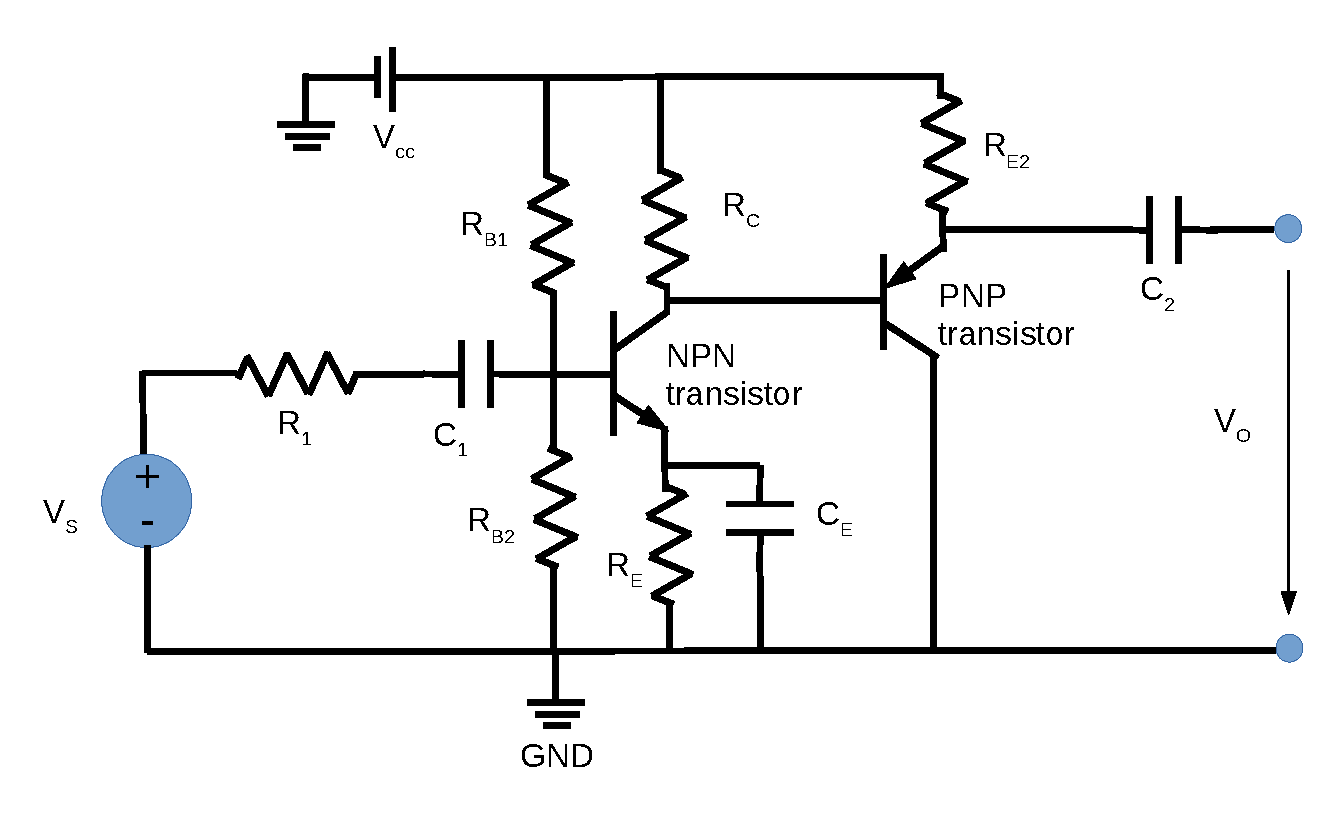
\includegraphics[scale=0.7]{lab4_principal.pdf}
    \caption{Circuit analysed.}
    \label{fig:circuito}
\end{figure}

The input ($V_{s}$) is a sinusoidal signal with a maximum amplitude of 10mV with an internal impendance of 100 $\Omega$, represented by $R_{in}$.
On the other end of the circuit we can find an 8 $\Omega$ speaker. Additionally, the circuit is supplied
by a 12V DC source, $V_{cc}$, that garantees that the transistor operates in its forward-active region (Base Biasing).

The gain stage mentioned, which is connected to the input signal, is formed by a single stage common-emitter amplifier
with degeneration that uses a NPN transistor. Furthermore, there is a bias circuit and a bypass capacitor which
functions will be discussed later in the report.
Moving on to the output stage, it was used a common collector amplifier but this time a PNP transistor was used.
This stage is basically responsible for lowering the output impendace that comes from the previous stage,
so that the values are appropriate for the speaker.

Now we will talk about the goal of the coupling capacitors ($C_{1}$ and $C_{2}$), bypass capacitors ($C_{3}$) and the effect of the resistance $R_{C}$.


Starting with the $C_{1}$ and $C_{2}$, they are low impendance coupling capacitors and DC blocking capacitors whose reactance at the signal frequency is designed to be negligible.
The AC coupling through capacitors is used to inject AC input signal and extract output signal without disturbing the Q-point (steady-state voltage or current at a specified terminal of an active device with no input signal applied.)
For this reason they have a direct impact on the lower and upper 3dB cut off frequencies and therefore the bandwidth of the network.

At low frequencies the reactance of coupling capacitor C2 is relatively high and hence very small part of the signal will pass from the amplifier stage to the load.
At high frequencies the reactance of coupling capacitor C2 is very small and it behaves as a short circuit. This increases the loading effect of the amplifier stage and serves to reduce the voltage gain.
At mid frequencies the voltage gain of the amplifier is constant. The effect of the coupling capacitor C2 in this frequency range is such as to maintain a constant voltage gain. Thus, as the frequency increases in this range, the reactance of C2 decreases, which tends to increase the gain.
If it is not used, then the amplified AC signal following through $R_{E}$ will cause a voltage drop across it, thereby dropping the output voltage.

$C_{3}$ is a bypass capacitor that provides a low impendace path for the AC current from emitter to ground,
thereby removing $R_{E}$ (required for good Q-point stability) from the circuit when AC signals are considered which garantees that the resistor will not affect the gain.

In Section~\ref{sec:analysis}, a theoretical analysis of the circuit is performed, followed by an simulation in \ref{sec:simulation}
with the goal of comparing and understand better the behaviour of this circuit.

%\begin{figure}[h] \centering
%    \includegraphics[scale=0.6]{}
%    \caption{Circuit analysed.}
%    \label{fig:rc}
%\end{figure}

%\begin{figure}[h] \centering
%    \includegraphics[scale=0.4]{}
%    \caption{Positive half.}
%    \label{fig:rc2}
%\end{figure}

%\begin{figure}[h] \centering
%    \includegraphics[scale=0.4]{}
%    \caption{Negative half.}
%    \label{fig:rc3}
%\end{figure}

%\begin{figure}[h] \centering
%    \includegraphics[scale=0.75]{}
%    \caption{Wave rectified.}
%    \label{fig:rc4}
%\end{figure}

%\begin{figure}[h] \centering
%    \includegraphics[scale=0.75]{}
%    \caption{Wave rectified, with filter.}
%    \label{fig:rc5}
%\end{figure}


